\documentclass{standalone}
\usepackage{tikz}
\usetikzlibrary{patterns, positioning}


\begin{document}
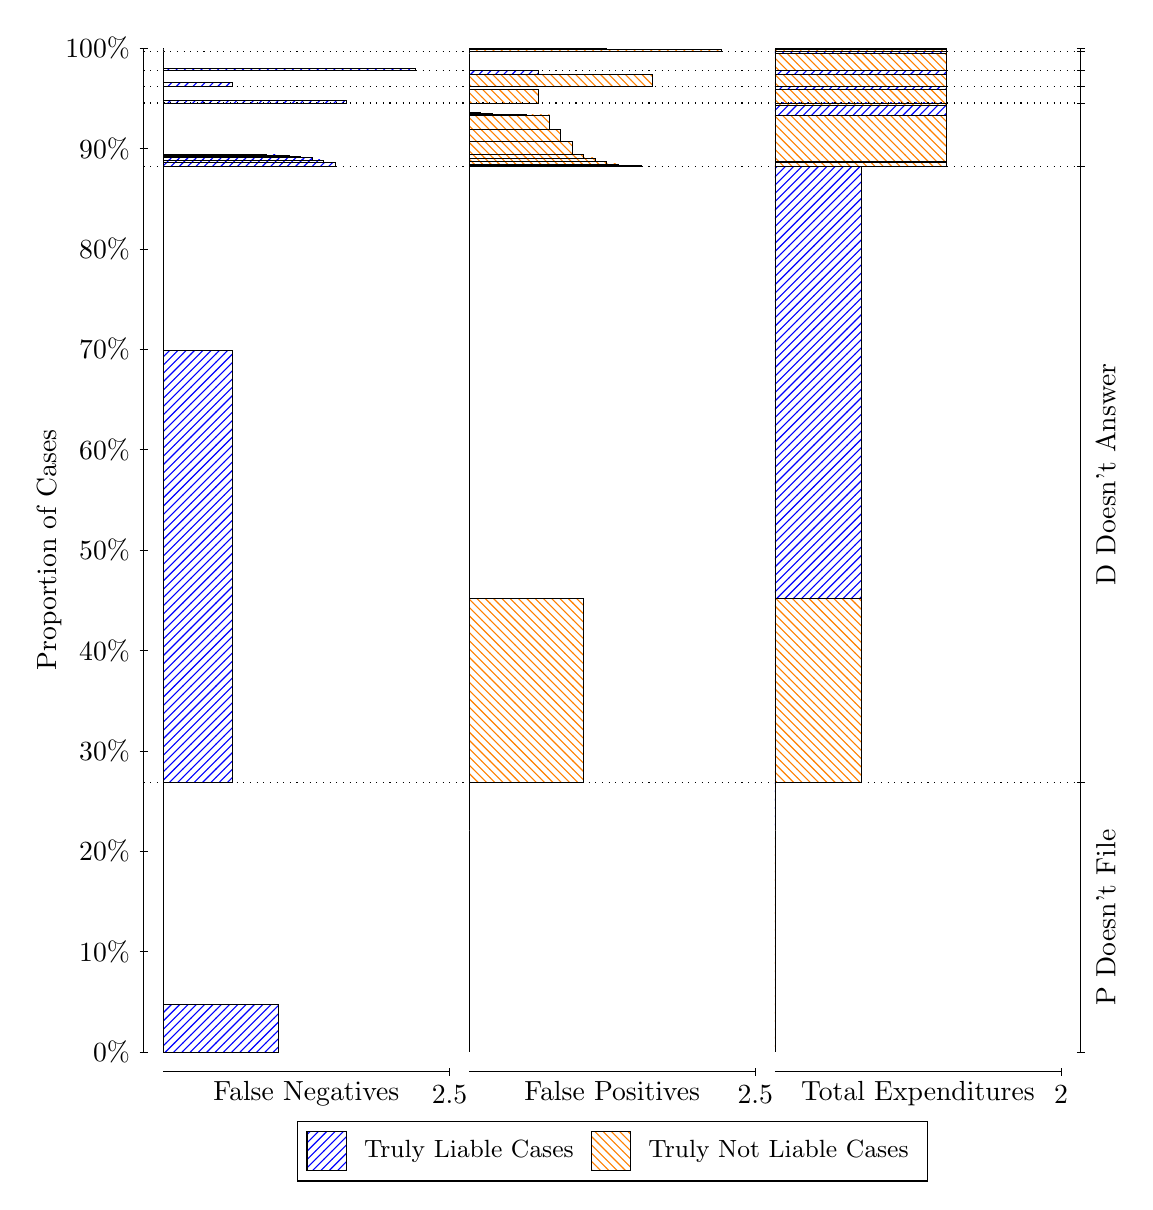
\begin{tikzpicture}
\draw[black, very thin] (1.5,1.75) -- (1.5,14.5);
\node[rotate=90, text=black, anchor=center] at (0.3, 8.125) {Proportion of Cases};
\draw[black, very thin] (1.45,1.75) -- (1.55,1.75);
\node[text=black, anchor=east] at (1.45, 1.75) {0\%};
\draw[black, very thin] (1.45,3.025) -- (1.55,3.025);
\node[text=black, anchor=east] at (1.45, 3.025) {10\%};
\draw[black, very thin] (1.45,4.3) -- (1.55,4.3);
\node[text=black, anchor=east] at (1.45, 4.3) {20\%};
\draw[black, very thin] (1.45,5.575) -- (1.55,5.575);
\node[text=black, anchor=east] at (1.45, 5.575) {30\%};
\draw[black, very thin] (1.45,6.85) -- (1.55,6.85);
\node[text=black, anchor=east] at (1.45, 6.85) {40\%};
\draw[black, very thin] (1.45,8.125) -- (1.55,8.125);
\node[text=black, anchor=east] at (1.45, 8.125) {50\%};
\draw[black, very thin] (1.45,9.4) -- (1.55,9.4);
\node[text=black, anchor=east] at (1.45, 9.4) {60\%};
\draw[black, very thin] (1.45,10.675) -- (1.55,10.675);
\node[text=black, anchor=east] at (1.45, 10.675) {70\%};
\draw[black, very thin] (1.45,11.95) -- (1.55,11.95);
\node[text=black, anchor=east] at (1.45, 11.95) {80\%};
\draw[black, very thin] (1.45,13.225) -- (1.55,13.225);
\node[text=black, anchor=east] at (1.45, 13.225) {90\%};
\draw[black, very thin] (1.45,14.5) -- (1.55,14.5);
\node[text=black, anchor=east] at (1.45, 14.5) {100\%};

\draw[black, very thin] (13.4,1.75) -- (13.4,14.5);
\draw[black, very thin] (13.35,1.75) -- (13.45,1.75);
\node[anchor=west] at (13.35, 1.75) {};
\draw[black, very thin] (13.35,5.1693) -- (13.45,5.1693);
\node[anchor=west] at (13.35, 5.1693) {};
\draw[black, very thin] (13.35,12.999) -- (13.45,12.999);
\node[anchor=west] at (13.35, 12.999) {};
\draw[black, very thin] (13.35,13.802) -- (13.45,13.802);
\node[anchor=west] at (13.35, 13.802) {};
\draw[black, very thin] (13.35,14.009) -- (13.45,14.009);
\node[anchor=west] at (13.35, 14.009) {};
\draw[black, very thin] (13.35,14.214) -- (13.45,14.214);
\node[anchor=west] at (13.35, 14.214) {};
\draw[black, very thin] (13.35,14.457) -- (13.45,14.457);
\node[anchor=west] at (13.35, 14.457) {};
\draw[black, very thin] (13.35,14.5) -- (13.45,14.5);
\node[anchor=west] at (13.35, 14.5) {};

\draw[black, very thin, pattern color=blue, pattern=north east lines] (1.75,1.75) rectangle (3.2033,2.3591);
\draw[black, very thin, pattern color=orange, pattern=north west lines] (1.75,2.3591) rectangle (1.75,5.1693);
\draw[black, very thin, pattern color=blue, pattern=north east lines] (1.75,5.1693) rectangle (2.622,10.659);
\draw[black, very thin, pattern color=orange, pattern=north west lines] (1.75,10.659) rectangle (1.75,12.999);
\draw[black, very thin, pattern color=blue, pattern=north east lines] (1.75,12.999) rectangle (3.93,13.046);
\draw[black, very thin, pattern color=blue, pattern=north east lines] (1.75,13.046) rectangle (3.7847,13.08);
\draw[black, very thin, pattern color=blue, pattern=north east lines] (1.75,13.08) rectangle (3.6393,13.113);
\draw[black, very thin, pattern color=blue, pattern=north east lines] (1.75,13.113) rectangle (3.494,13.123);
\draw[black, very thin, pattern color=blue, pattern=north east lines] (1.75,13.123) rectangle (3.3487,13.135);
\draw[black, very thin, pattern color=blue, pattern=north east lines] (1.75,13.135) rectangle (3.2033,13.142);
\draw[black, very thin, pattern color=blue, pattern=north east lines] (1.75,13.142) rectangle (3.058,13.146);
\draw[black, very thin, pattern color=blue, pattern=north east lines] (1.75,13.146) rectangle (2.9127,13.148);
\draw[black, very thin, pattern color=blue, pattern=north east lines] (1.75,13.148) rectangle (2.7673,13.15);
\draw[black, very thin, pattern color=orange, pattern=north west lines] (1.75,13.15) rectangle (1.75,13.802);
\draw[black, very thin, pattern color=blue, pattern=north east lines] (1.75,13.802) rectangle (4.0753,13.833);
\draw[black, very thin, pattern color=orange, pattern=north west lines] (1.75,13.833) rectangle (1.75,14.009);
\draw[black, very thin, pattern color=blue, pattern=north east lines] (1.75,14.009) rectangle (2.622,14.059);
\draw[black, very thin, pattern color=orange, pattern=north west lines] (1.75,14.059) rectangle (1.75,14.214);
\draw[black, very thin, pattern color=blue, pattern=north east lines] (1.75,14.214) rectangle (4.9473,14.241);
\draw[black, very thin, pattern color=orange, pattern=north west lines] (1.75,14.241) rectangle (1.75,14.457);
\draw[black, very thin, pattern color=orange, pattern=north west lines] (1.75,14.457) rectangle (1.75,14.483);
\draw[black, very thin, pattern color=blue, pattern=north east lines] (1.75,14.483) rectangle (1.75,14.5);
\draw[black, very thin, pattern color=orange, pattern=north west lines] (5.6333,1.75) rectangle (5.6333,4.5601);
\draw[black, very thin, pattern color=blue, pattern=north east lines] (5.6333,4.5601) rectangle (5.6333,5.1693);
\draw[black, very thin, pattern color=orange, pattern=north west lines] (5.6333,5.1693) rectangle (7.0867,7.5096);
\draw[black, very thin, pattern color=blue, pattern=north east lines] (5.6333,7.5096) rectangle (5.6333,12.999);
\draw[black, very thin, pattern color=orange, pattern=north west lines] (5.6333,12.999) rectangle (7.8133,13.006);
\draw[black, very thin, pattern color=orange, pattern=north west lines] (5.6333,13.006) rectangle (7.668,13.013);
\draw[black, very thin, pattern color=orange, pattern=north west lines] (5.6333,13.013) rectangle (7.5227,13.028);
\draw[black, very thin, pattern color=orange, pattern=north west lines] (5.6333,13.028) rectangle (7.3773,13.057);
\draw[black, very thin, pattern color=orange, pattern=north west lines] (5.6333,13.057) rectangle (7.232,13.106);
\draw[black, very thin, pattern color=orange, pattern=north west lines] (5.6333,13.106) rectangle (7.0867,13.145);
\draw[black, very thin, pattern color=orange, pattern=north west lines] (5.6333,13.145) rectangle (6.9413,13.318);
\draw[black, very thin, pattern color=orange, pattern=north west lines] (5.6333,13.318) rectangle (6.796,13.463);
\draw[black, very thin, pattern color=orange, pattern=north west lines] (5.6333,13.463) rectangle (6.6507,13.651);
\draw[black, very thin, pattern color=blue, pattern=north east lines] (5.6333,13.651) rectangle (6.36,13.653);
\draw[black, very thin, pattern color=blue, pattern=north east lines] (5.6333,13.653) rectangle (6.2147,13.655);
\draw[black, very thin, pattern color=blue, pattern=north east lines] (5.6333,13.655) rectangle (6.0693,13.659);
\draw[black, very thin, pattern color=blue, pattern=north east lines] (5.6333,13.659) rectangle (5.924,13.666);
\draw[black, very thin, pattern color=blue, pattern=north east lines] (5.6333,13.666) rectangle (5.7787,13.678);
\draw[black, very thin, pattern color=blue, pattern=north east lines] (5.6333,13.678) rectangle (5.6333,13.802);
\draw[black, very thin, pattern color=orange, pattern=north west lines] (5.6333,13.802) rectangle (6.5053,13.978);
\draw[black, very thin, pattern color=blue, pattern=north east lines] (5.6333,13.978) rectangle (5.6333,14.009);
\draw[black, very thin, pattern color=orange, pattern=north west lines] (5.6333,14.009) rectangle (7.9587,14.164);
\draw[black, very thin, pattern color=blue, pattern=north east lines] (5.6333,14.164) rectangle (6.5053,14.214);
\draw[black, very thin, pattern color=orange, pattern=north west lines] (5.6333,14.214) rectangle (5.6333,14.43);
\draw[black, very thin, pattern color=blue, pattern=north east lines] (5.6333,14.43) rectangle (5.6333,14.457);
\draw[black, very thin, pattern color=orange, pattern=north west lines] (5.6333,14.457) rectangle (8.8307,14.483);
\draw[black, very thin, pattern color=blue, pattern=north east lines] (5.6333,14.483) rectangle (7.3773,14.5);
\draw[black, very thin, pattern color=orange, pattern=north west lines] (9.5167,1.75) rectangle (9.5167,4.5601);
\draw[black, very thin, pattern color=blue, pattern=north east lines] (9.5167,4.5601) rectangle (9.5167,5.1693);
\draw[black, very thin, pattern color=orange, pattern=north west lines] (9.5167,5.1693) rectangle (10.607,7.5096);
\draw[black, very thin, pattern color=blue, pattern=north east lines] (9.5167,7.5096) rectangle (10.607,12.999);
\draw[black, very thin, pattern color=orange, pattern=north west lines] (9.5167,12.999) rectangle (11.697,13.048);
\draw[black, very thin, pattern color=blue, pattern=north east lines] (9.5167,13.048) rectangle (11.697,13.06);
\draw[black, very thin, pattern color=orange, pattern=north west lines] (9.5167,13.06) rectangle (11.697,13.641);
\draw[black, very thin, pattern color=blue, pattern=north east lines] (9.5167,13.641) rectangle (11.697,13.773);
\draw[black, very thin, pattern color=orange, pattern=north west lines] (9.5167,13.773) rectangle (11.697,13.795);
\draw[black, very thin, pattern color=blue, pattern=north east lines] (9.5167,13.795) rectangle (11.697,13.802);
\draw[black, very thin, pattern color=orange, pattern=north west lines] (9.5167,13.802) rectangle (11.697,13.978);
\draw[black, very thin, pattern color=blue, pattern=north east lines] (9.5167,13.978) rectangle (11.697,14.009);
\draw[black, very thin, pattern color=orange, pattern=north west lines] (9.5167,14.009) rectangle (11.697,14.164);
\draw[black, very thin, pattern color=blue, pattern=north east lines] (9.5167,14.164) rectangle (11.697,14.214);
\draw[black, very thin, pattern color=orange, pattern=north west lines] (9.5167,14.214) rectangle (11.697,14.43);
\draw[black, very thin, pattern color=blue, pattern=north east lines] (9.5167,14.43) rectangle (11.697,14.457);
\draw[black, very thin, pattern color=orange, pattern=north west lines] (9.5167,14.457) rectangle (11.697,14.483);
\draw[black, very thin, pattern color=blue, pattern=north east lines] (9.5167,14.483) rectangle (11.697,14.5);
\draw[black, dotted] (1.5,5.1693) -- (13.4,5.1693);
\draw[black, dotted] (1.5,12.999) -- (13.4,12.999);
\draw[black, dotted] (1.5,13.802) -- (13.4,13.802);
\draw[black, dotted] (1.5,14.009) -- (13.4,14.009);
\draw[black, dotted] (1.5,14.214) -- (13.4,14.214);
\draw[black, dotted] (1.5,14.457) -- (13.4,14.457);
\draw[black, very thin] (1.75,1.5) -- (5.3833,1.5);
\node[text=black, anchor=north] at (3.5667, 1.5) {False Negatives};
\draw[black, very thin] (5.3833,1.45) -- (5.3833,1.55);
\node[text=black, anchor=north] at (5.3833, 1.45) {2.5};

\draw[black, very thin] (5.6333,1.5) -- (9.2667,1.5);
\node[text=black, anchor=north] at (7.45, 1.5) {False Positives};
\draw[black, very thin] (9.2667,1.45) -- (9.2667,1.55);
\node[text=black, anchor=north] at (9.2667, 1.45) {2.5};

\draw[black, very thin] (9.5167,1.5) -- (13.15,1.5);
\node[text=black, anchor=north] at (11.333, 1.5) {Total Expenditures};
\draw[black, very thin] (13.15,1.45) -- (13.15,1.55);
\node[text=black, anchor=north] at (13.15, 1.45) {2};

\node[text=black, centered, rotate=90] at (13.72, 3.4596) {P Doesn't File};
\node[text=black, centered, rotate=90] at (13.72, 9.0841) {D Doesn't Answer};






\draw (7.449999999999999,1.5) node[draw=none] (baseCoordinate) {};
\begin{scope}[align=center]
        \matrix[scale=0.5, draw=black, below=0.5cm of baseCoordinate, nodes={draw}, column sep=0.1cm]{
            \node[rectangle, draw, minimum width=0.5cm, minimum height=0.5cm, pattern color=blue, pattern=north east lines] {}; &
            \node[draw=none, font=\small, text=black] (B) {Truly Liable Cases}; &
            \node[rectangle, draw, minimum width=0.5cm, minimum height=0.5cm, pattern color=orange, pattern=north west lines] {}; &
            \node[draw=none, font=\small, text=black] (B) {Truly Not Liable Cases}; \\
            };
\end{scope}

\end{tikzpicture}
\end{document}